\documentclass{article}
\usepackage{xcolor}
\usepackage{titleps}
\usepackage[letterpaper, margin=0.95in]{geometry}
\usepackage{url}
\usepackage{amsmath}
\usepackage{amssymb}
\usepackage{wrapfig}
\usepackage{float}
\usepackage{mathtools}
\usepackage{enumitem}
\usepackage{tabu}
\usepackage{parskip}
\usepackage{natbib}
\usepackage{listings}

\usepackage[many]{tcolorbox}
\usepackage{minted}
\setminted[python]{
	% frame=single,
	% linenos,
    xleftmargin=0.475em,
    baselinestretch=1.2,
}
% https://tex.stackexchange.com/a/569249
\setcounter{secnumdepth}{5}
\setcounter{tocdepth}{5}
\makeatletter
\newcommand\subsubsubsection{\@startsection{paragraph}{4}{\z@}{-2.5ex\@plus -1ex \@minus -.25ex}{1.25ex \@plus .25ex}{\normalfont\normalsize\bfseries}}
\newcommand\subsubsubsubsection{\@startsection{subparagraph}{5}{\z@}{-2.5ex\@plus -1ex \@minus -.25ex}{1.25ex \@plus .25ex}{\normalfont\normalsize\bfseries}}
\makeatother

\usepackage{hyperref}
\usepackage[color=red]{todonotes}
\usepackage{forest}
\definecolor{light-yellow}{HTML}{FFE5CC}

\newpagestyle{ruled}
{\sethead{CMU 16-831}{Introduction to Robot Learning }{Spring 2024}\headrule
  \setfoot{}{}{}}
\pagestyle{ruled}

\renewcommand\makeheadrule{\color{black}\rule[-.75\baselineskip]{\linewidth}{0.4pt}}
\renewcommand*\footnoterule{}

\newtcolorbox[]{answer}[1][]{
    % breakable,
    enhanced,
    nobeforeafter,
    colback=white,
    title=Your Answer,
    sidebyside align=top,
    box align=top,
    #1
}



\begin{document}

\lstset{basicstyle = \ttfamily,columns=fullflexible,
backgroundcolor = \color{light-yellow}
}

\begin{centering}
    {\Large Assignment 2: Policy Gradient} \\
    \vspace{.25cm}
    % \textbf{Due September 13, 11:59 pm} \\
\end{centering}
\vspace{0.25cm}

\textbf{Andrew ID:} \texttt{lzaceria} \\
\textbf{Collaborators:} \texttt{Write the Andrew IDs of your collaborators here (if any).}\\ 
\textbf{NOTE:} Please do \textbf{NOT} change the sizes of the answer blocks or plots.

\setcounter{section}{4}
\section{Small-Scale Experiments}

\subsection{Experiment 1 (Cartpole) -- \lbrack5 points total\rbrack}

\subsubsection{Configurations}
\begin{answer}[title=Q5.1.1,height=6cm,width=\linewidth]
% TODO
\begin{minted}
[framesep=2mm, fontsize=\scriptsize, breaklines]
{bash}
python rob831/scripts/run_hw2.py --env_name CartPole-v0 -n 150 -b 1500 \
    -dsa --exp_name q1_sb_no_rtg_dsa

python rob831/scripts/run_hw2.py --env_name CartPole-v0 -n 150 -b 1500 \
    -rtg -dsa --exp_name q1_sb_rtg_dsa

python rob831/scripts/run_hw2.py --env_name CartPole-v0 -n 150 -b 1500 \
    -rtg --exp_name q1_sb_rtg_na

python rob831/scripts/run_hw2.py --env_name CartPole-v0 -n 150 -b 6000 \
    -dsa --exp_name q1_lb_no_rtg_dsa

python rob831/scripts/run_hw2.py --env_name CartPole-v0 -n 150 -b 6000 \
    -rtg -dsa --exp_name q1_lb_rtg_dsa

python rob831/scripts/run_hw2.py --env_name CartPole-v0 -n 150 -b 6000 \
    -rtg --exp_name q1_lb_rtg_na
\end{minted}
\end{answer}

\subsubsection{Plots}

\subsubsubsection{Small batch -- \lbrack1 points\rbrack}
\begin{answer}[title=Q5.1.2.1,height=9.5cm,width=\linewidth]
\centering
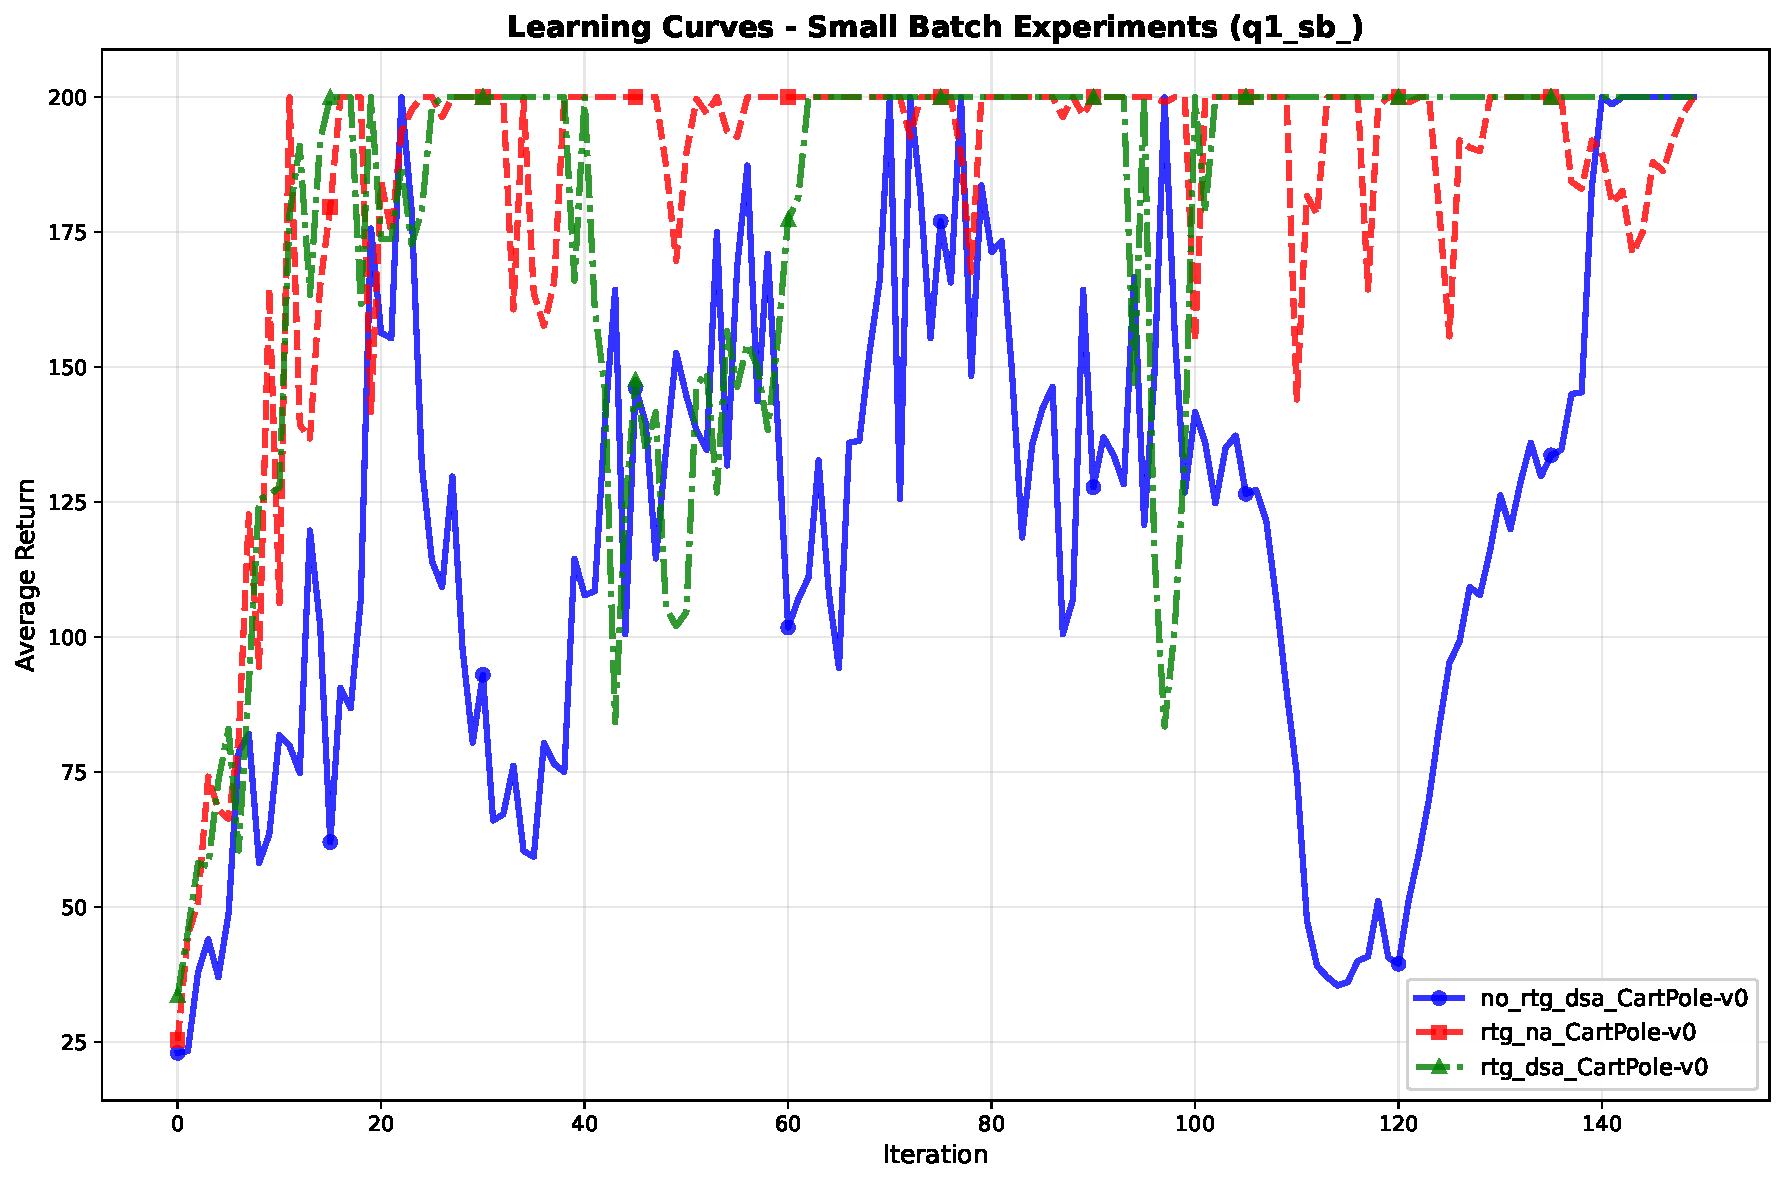
\includegraphics[height=8cm]{plots_submission/small_batch_learning_curves.pdf}
\end{answer}

\subsubsubsection{Large batch -- \lbrack1 points\rbrack}
\begin{answer}[title=Q5.1.2.2,height=9.5cm,width=\linewidth]
\centering
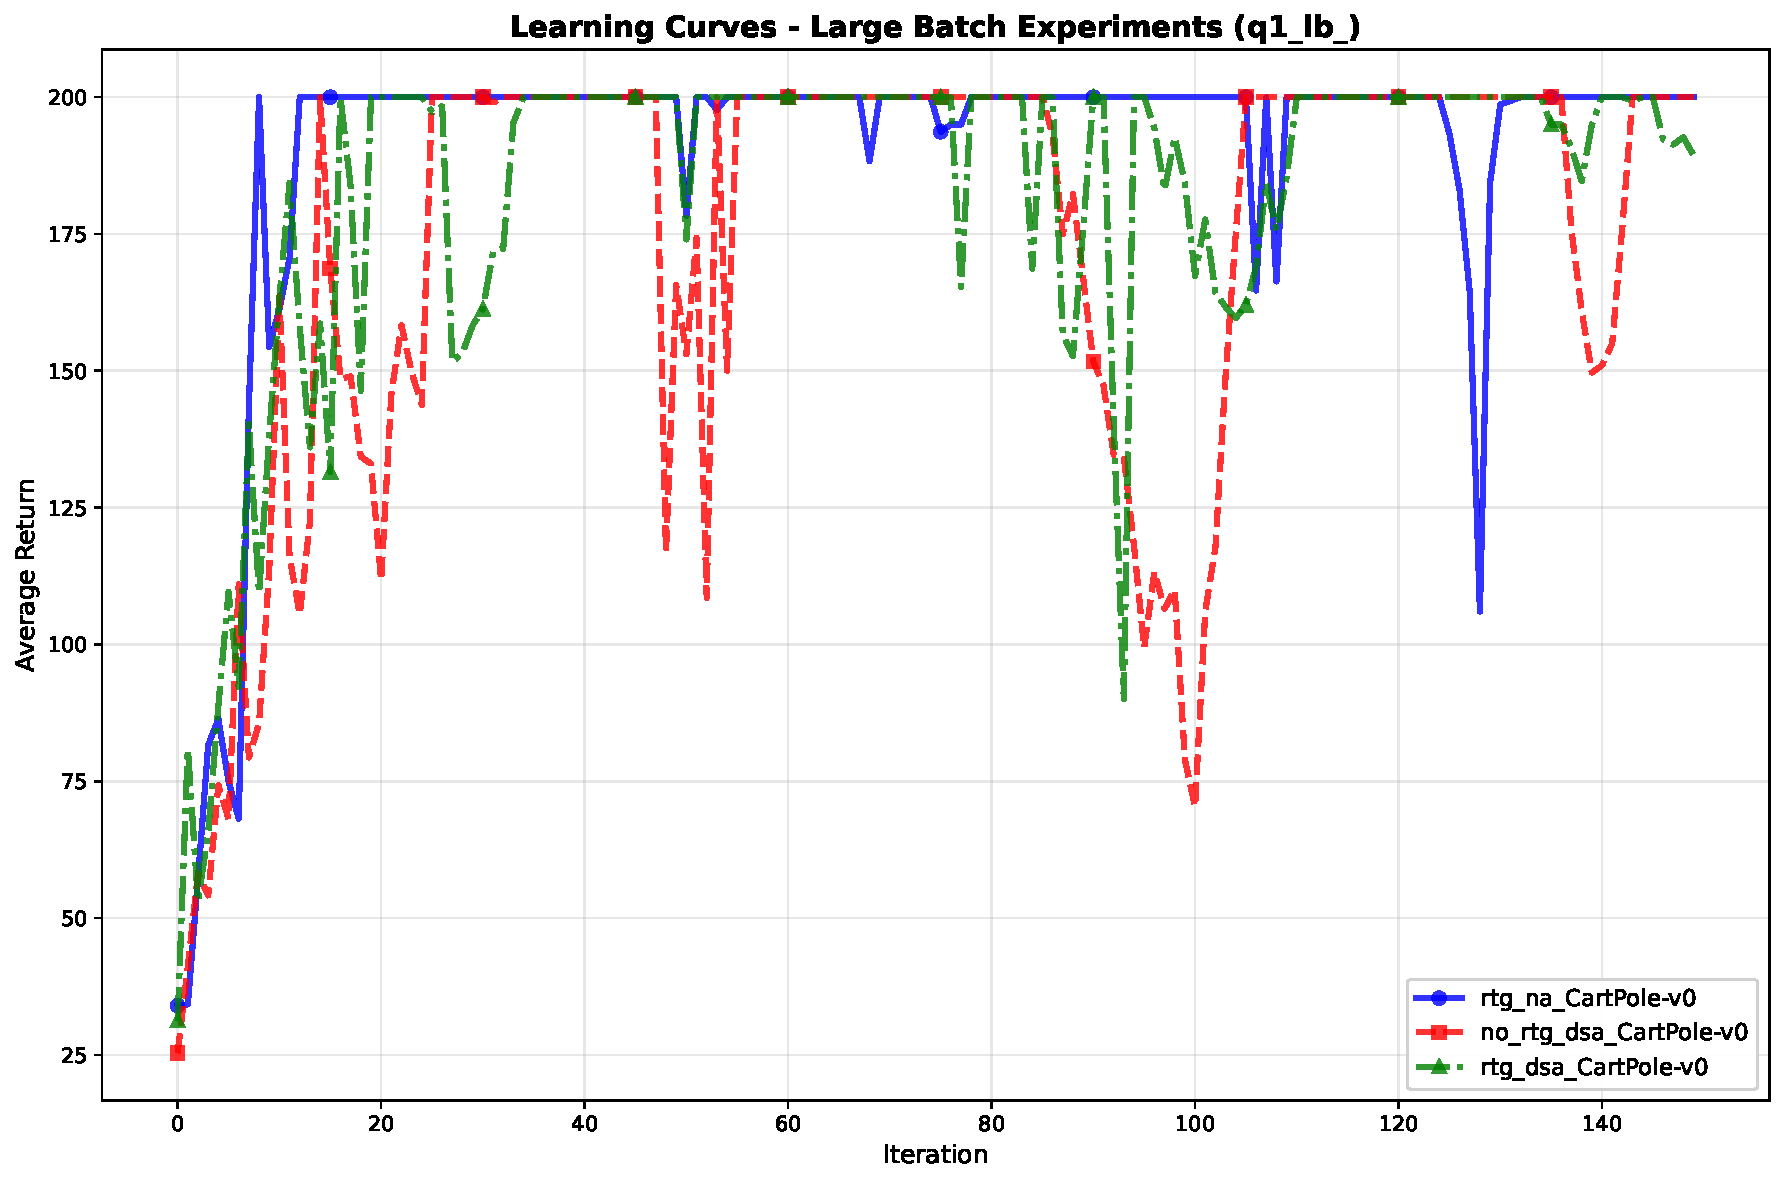
\includegraphics[height=8cm]{plots_submission/large_batch_learning_curves.pdf}
\end{answer}

\subsubsection{Analysis}

\subsubsubsection{Value estimator -- \lbrack1 points\rbrack}
\begin{answer}[title=Q5.1.3.1,height=4cm,width=\linewidth]
Reward-to-go performs better than trajectory-centric.
\end{answer}

\subsubsubsection{Advantage standardization -- \lbrack1 points\rbrack}
\begin{answer}[title=Q5.1.3.2,height=4cm,width=\linewidth]
Yes, advantage standardization helped.
\end{answer}

\subsubsubsection{Batch size -- \lbrack1 points\rbrack}
\begin{answer}[title=Q5.1.3.3,height=4cm,width=\linewidth]
Yes, the batch size made an impact. A bigger batch size generally improves performance.
\end{answer}

\subsection{Experiment 2 (InvertedPendulum) -- \lbrack4 points total\rbrack}

\subsubsection{Configurations -- \lbrack1.5 points\rbrack}
\begin{answer}[title=Q5.2.1,height=10cm,width=\linewidth]
\begin{minted}
[framesep=2mm, fontsize=\scriptsize, breaklines]
{bash}
python rob831/scripts/run_hw2.py \
    --env_name InvertedPendulum-v4 \
    --ep_len 1000 \
    --discount 0.92 \
    -n 100 \
    -l 2 \
    -s 64 \
    -b 50 \
    -lr 0.02 \
    -rtg \
    --exp_name q2_b50_r0.02_test
python rob831/scripts/run_hw2.py \
    --env_name InvertedPendulum-v4 \
    --ep_len 1000 \
    --discount 0.92 \
    -n 100 \
    -l 2 \
    -s 64 \
    -b 40 \
    -lr 0.02 \
    -rtg \
    --exp_name q2_b40_r0.02_test
python rob831/scripts/run_hw2.py \
    --env_name InvertedPendulum-v4 \
    --ep_len 1000 \
    --discount 0.92 \
    -n 100 \
    -l 2 \
    -s 64 \
    -b 50 \
    -lr 0.01 \
    -rtg \
    --exp_name q2_b50_r0.01_test

\end{minted}
\end{answer}

\subsubsection{smallest \textbf{b*} and largest \textbf{r*} (same run) -- \lbrack1.5 points\rbrack}
\begin{answer}[title=Q5.2.2,height=4cm,width=\linewidth]
b*=50, r*=0.02
\end{answer}

\subsubsection{Plot -- \lbrack1 points\rbrack}
\begin{answer}[title=Q5.2.3,height=10cm,width=\linewidth]
    \centering
    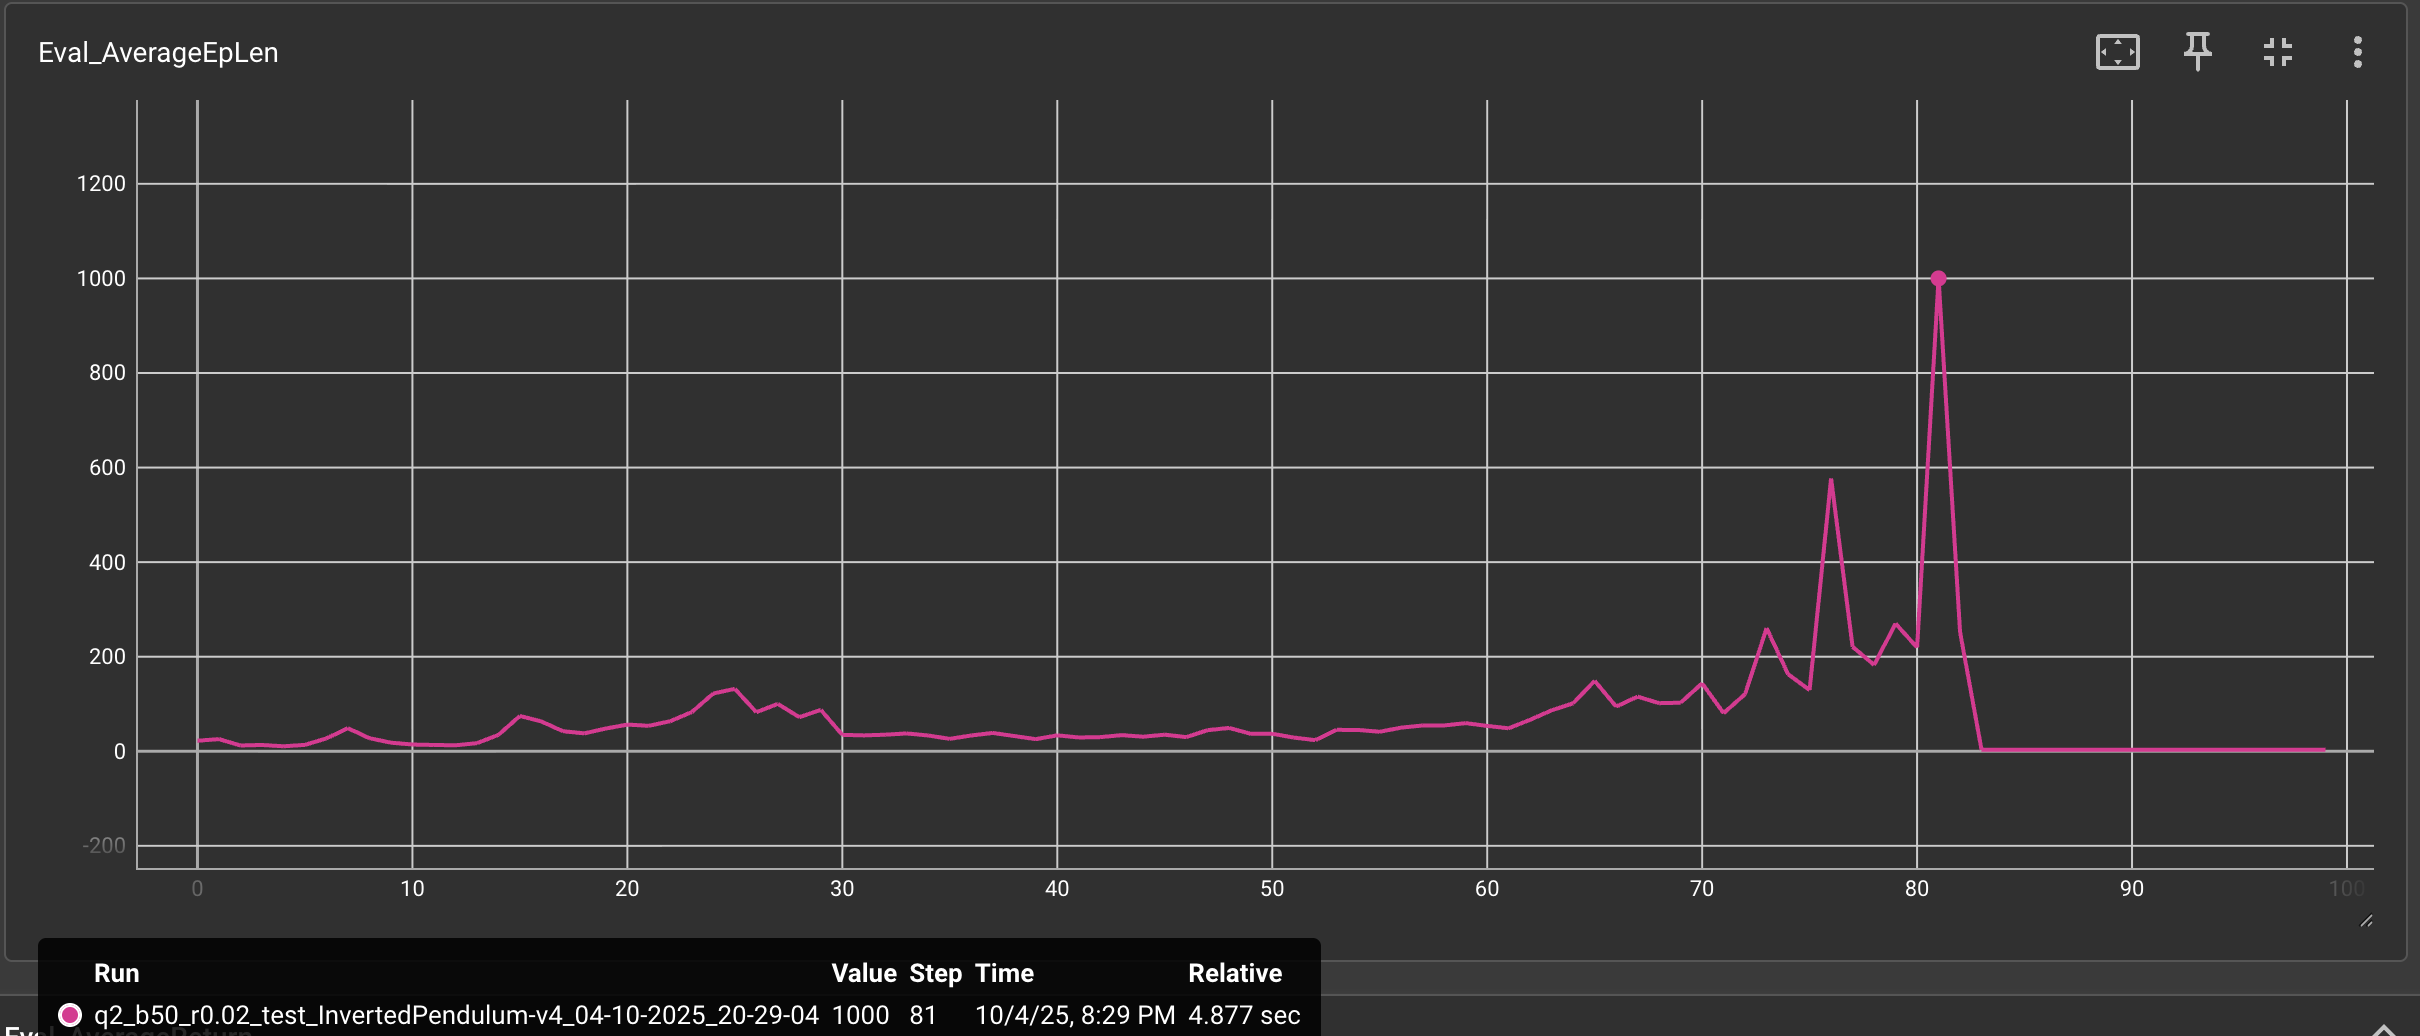
\includegraphics[height=8cm, width=\linewidth]{plots_submission/section5_exp2_plot.png}
\end{answer}

\setcounter{section}{6}
\section{More Complex Experiments}

\subsection{Experiment 3 (LunarLander) -- \lbrack1 points total\rbrack}

\subsubsection{Configurations}
\begin{answer}[title=Q7.1.1,height=6cm,width=\linewidth]
\begin{minted}
[framesep=2mm, fontsize=\scriptsize, breaklines]
{bash}
Had to switch to v3
python rob831/scripts/run_hw2.py \
    --env_name LunarLanderContinuous-v3 --ep_len 1000
    --discount 0.99 -n 100 -l 2 -s 64 -b 10000 -lr 0.005 \
    --reward_to_go --nn_baseline --exp_name q3_b10000_r0.005
\end{minted}
\end{answer}

\subsubsection{Plot -- \lbrack1 points\rbrack}
\begin{answer}[title=Q7.1.2,height=10cm,width=\linewidth]
% TODO
\centering
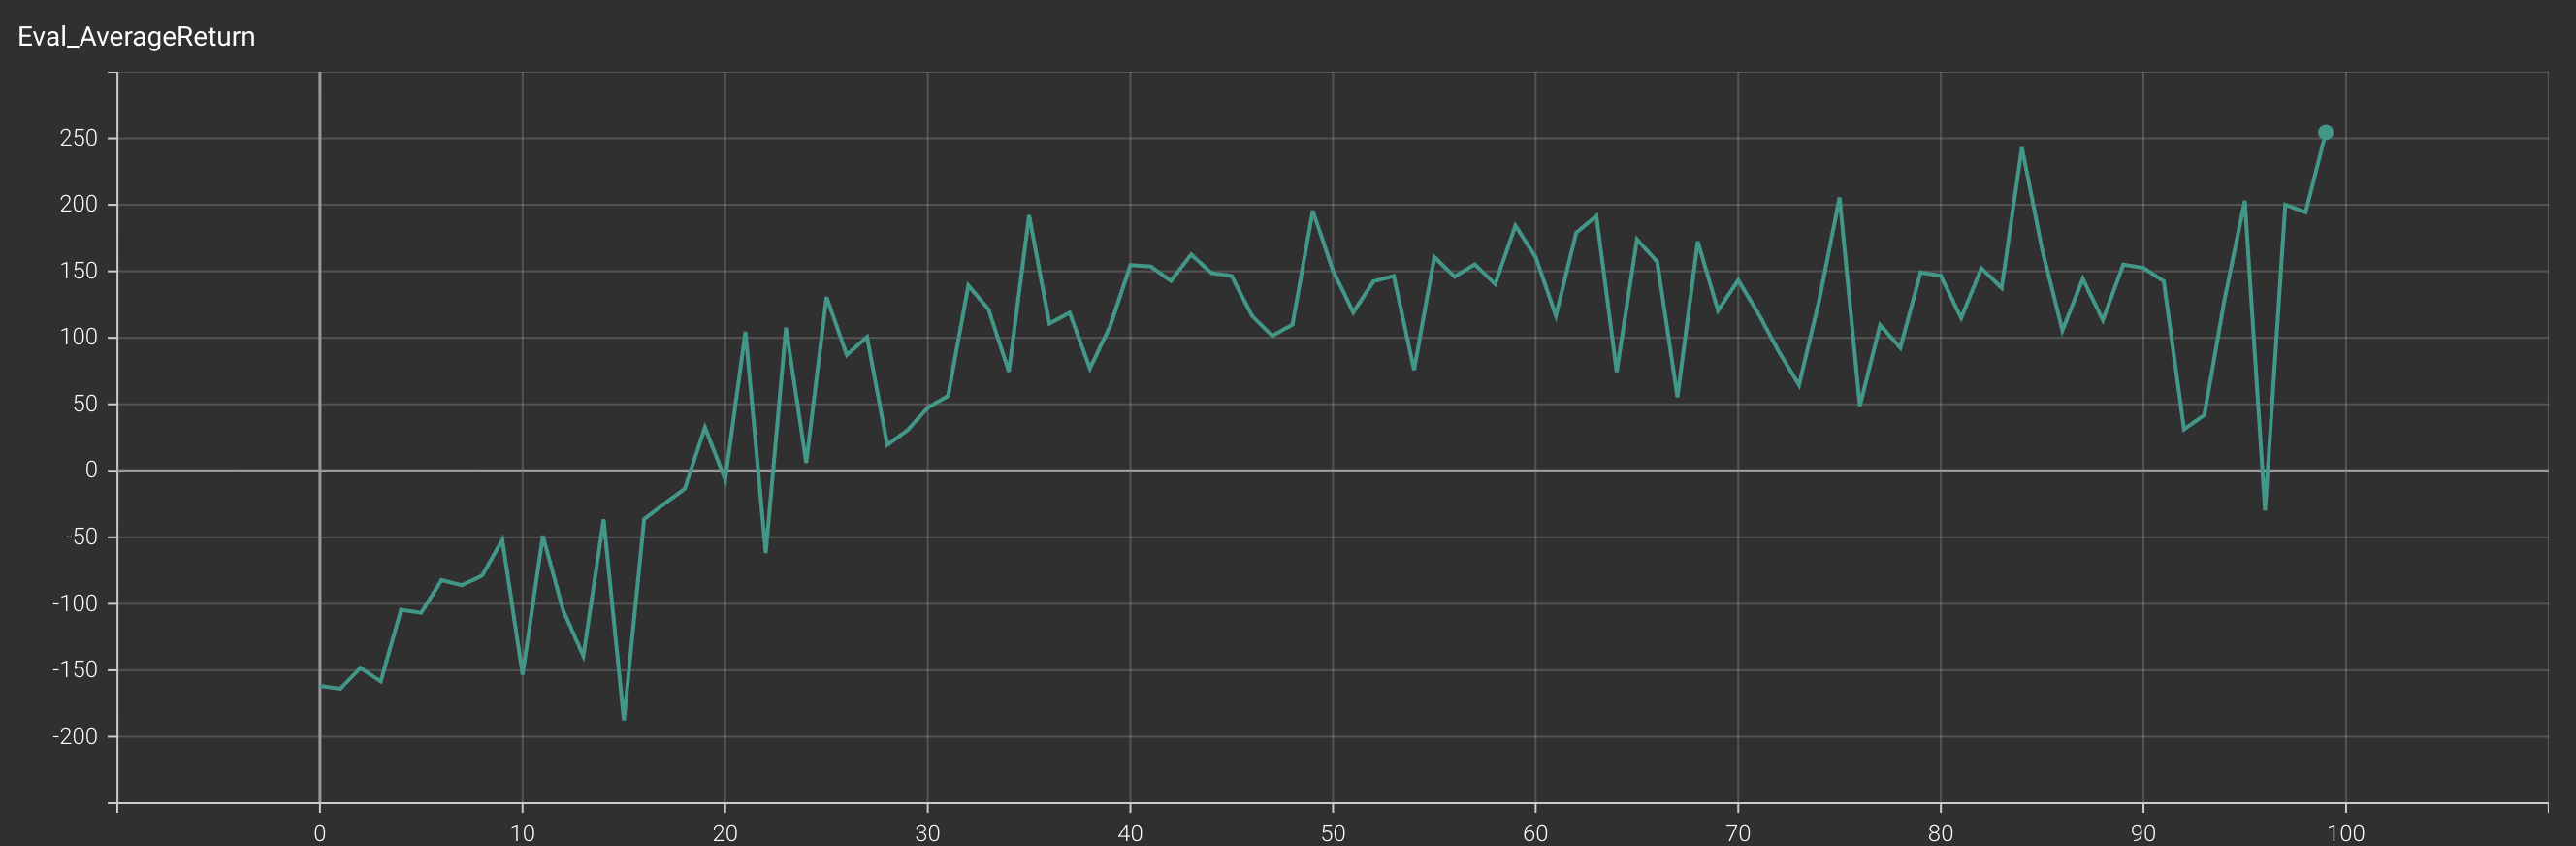
\includegraphics[height=8cm,width=\linewidth]{plots_submission/section7_exp3_lunarlander_plot.png}
\end{answer}

\subsection{Experiment 4 (HalfCheetah) -- \lbrack1 points\rbrack}

\subsubsection{Configurations}
\begin{answer}[title=Q7.2.1,height=10cm,width=\linewidth]
\begin{minted}
[framesep=2mm, fontsize=\scriptsize, breaklines, escapeinside=||, mathescape=true]
{python}
python rob831/scripts/run_hw2.py --env_name HalfCheetah-v4 --ep_len 150 \
    --discount 0.95 -n 100 -l 2 -s 32 -b 10000 -lr 0.02 \
    --exp_name q4_search_b10000_lr0.02
python rob831/scripts/run_hw2.py --env_name HalfCheetah-v4 --ep_len 150 \
    --discount 0.95 -n 100 -l 2 -s 32 -b 10000 -lr 0.02 -rtg \
    --exp_name q4_search_b10000_lr0.02_rtg
python rob831/scripts/run_hw2.py --env_name HalfCheetah-v4 --ep_len 150 \
    --discount 0.95 -n 100 -l 2 -s 32 -b 10000 -lr 0.02 --nn_baseline \
    --exp_name q4_search_b10000_lr0.02_nnbaseline
python rob831/scripts/run_hw2.py --env_name HalfCheetah-v4 --ep_len 150 \
    --discount 0.95 -n 100 -l 2 -s 32 -b 10000 -lr 0.02 -rtg --nn_baseline \
    --exp_name q4_search_b10000_lr0.02_rtg_nnbaseline
\end{minted}
\end{answer}

\subsubsection{Plot -- \lbrack1 points\rbrack}
\begin{answer}[title=Q7.2.2,height=10cm,width=\linewidth]
% TODO
\centering
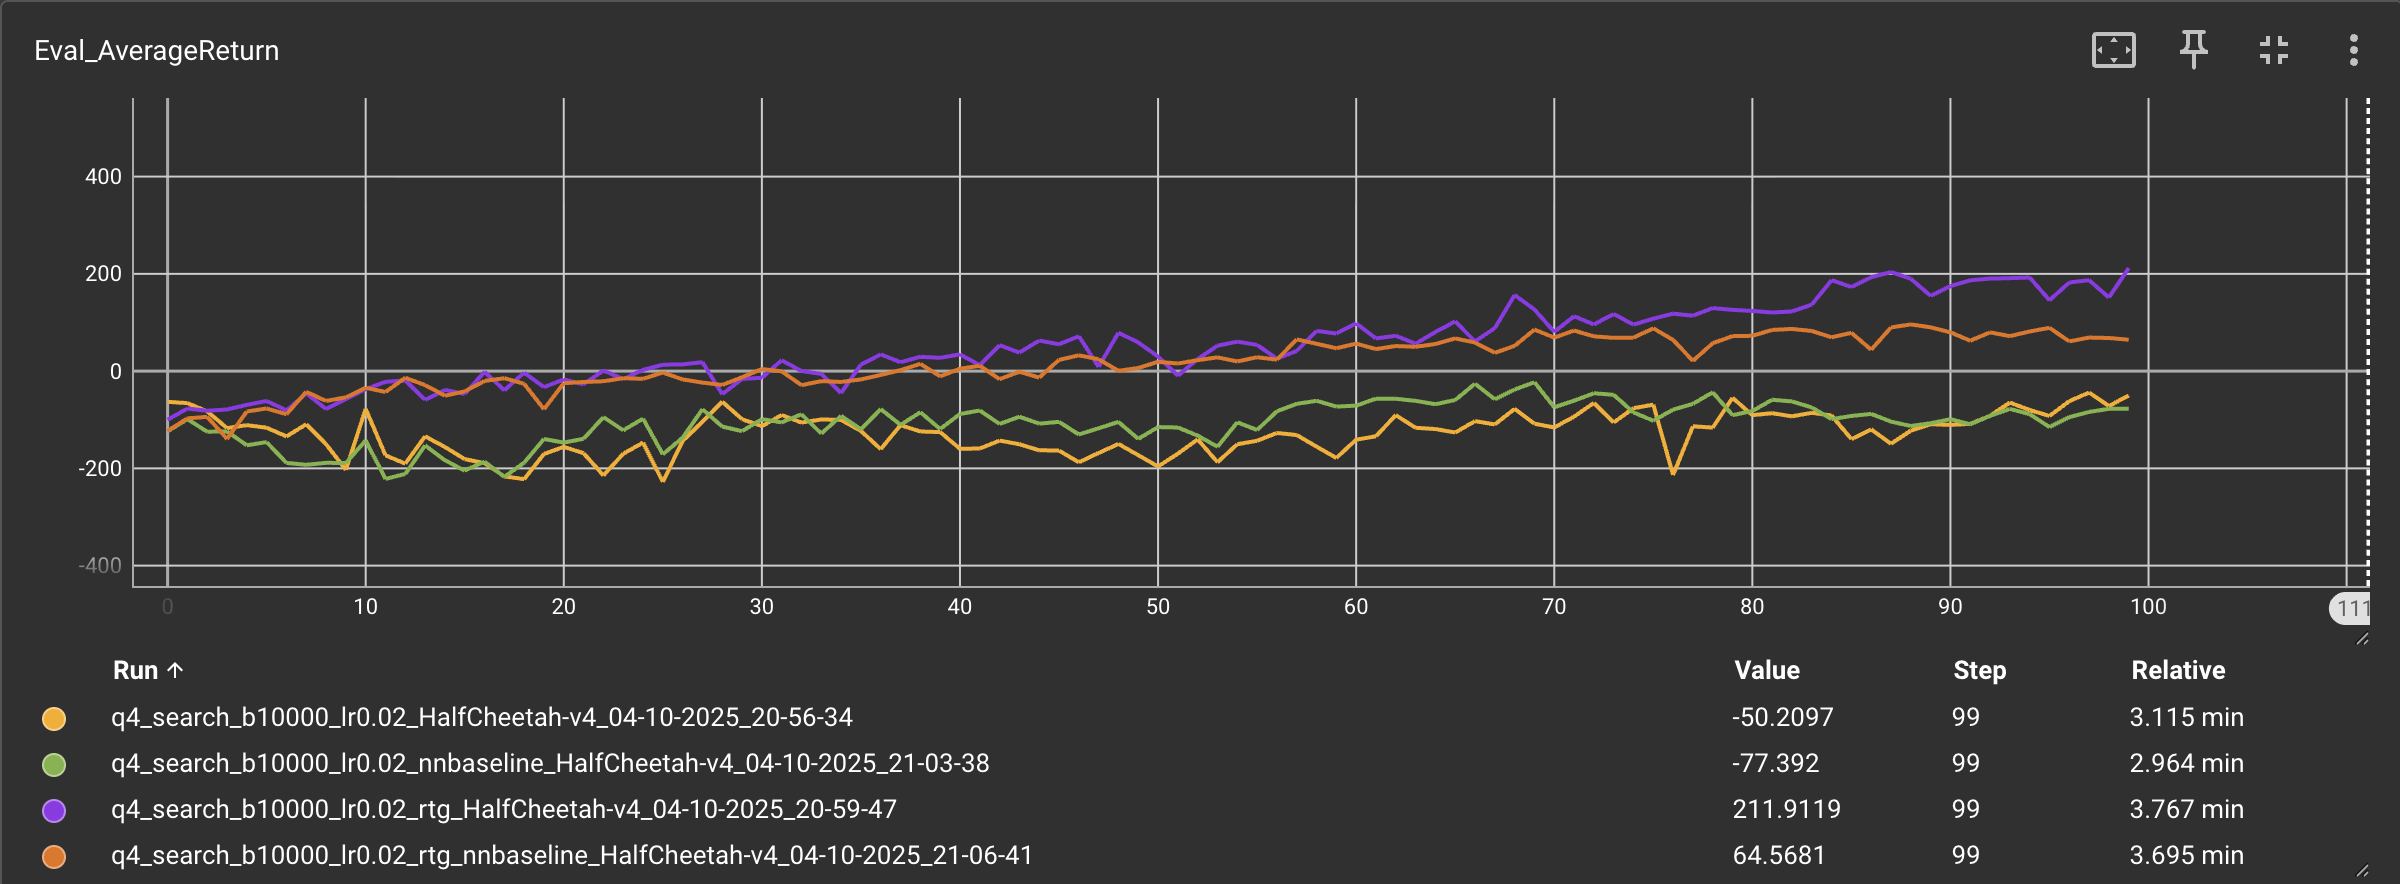
\includegraphics[height=8cm,width=\linewidth]{plots_submission/7_2_2_plot.png}
\end{answer}

\subsubsection{ Optimal b* and r* -- \lbrack0.5 points\rbrack}
\begin{answer}[title=Q7.2.3,height=4cm,width=\linewidth]
b15000, r0.02
\end{answer}

\subsubsection{ Plot -- \lbrack0.5 points\rbrack}
\begin{answer}[title=Q7.2.4,height=10cm,width=\linewidth]
% TODO
\centering
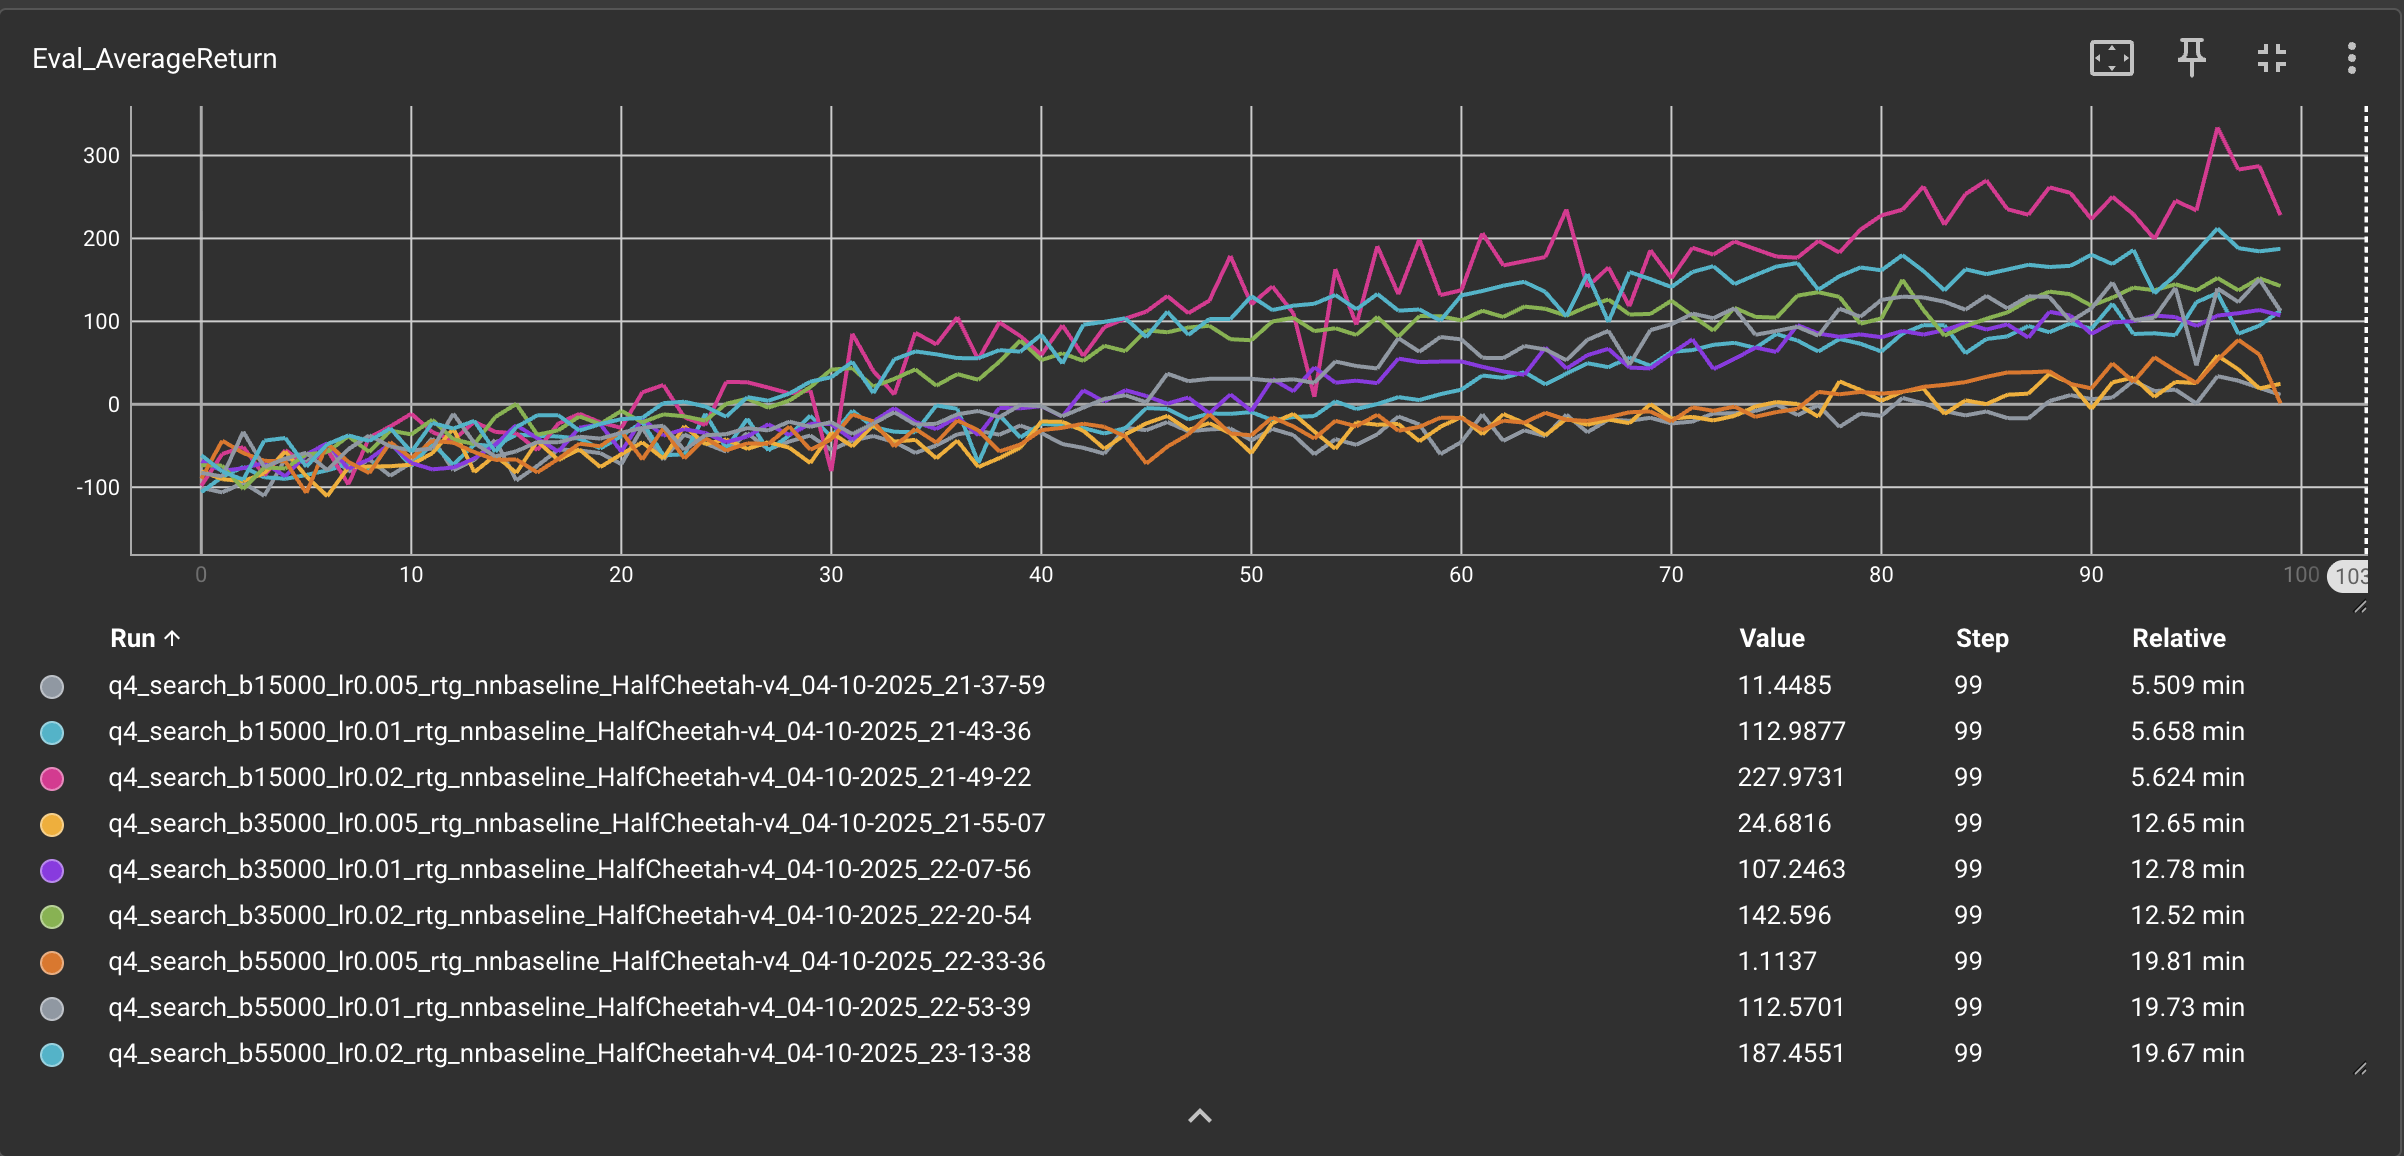
\includegraphics[height=8cm,width=\linewidth]{plots_submission/7_2_4_plot.png}
\end{answer}

\subsubsection{ Describe how b* and r* affect task performance -- \lbrack0.5 points\rbrack}
\begin{answer}[title=Q7.2.5,height=4cm,width=\linewidth]
A higher learning rate r* generally improves performance, while b* does not change performance much if comparing with the same r*.
\end{answer}

\subsubsection{Configurations with optimal b* and r* -- \lbrack0.5 points\rbrack}
\begin{answer}[title=Q7.2.6,height=6cm,width=\linewidth]
% TODO
\begin{minted}
[framesep=2mm, fontsize=\scriptsize, breaklines]
{bash}
python rob831/scripts/run_hw2.py --env_name HalfCheetah-v4 --ep_len 150 \
    --discount 0.95 -n 100 -l 2 -s 32 -b b15000 -lr 0.02 \
    --exp_name q4_b15000_r0.02

python rob831/scripts/run_hw2.py --env_name HalfCheetah-v4 --ep_len 150 \
    --discount 0.95 -n 100 -l 2 -s 32 -b b15000 -lr 0.02 -rtg \
    --exp_name q4_b15000_r0.02_rtg

python rob831/scripts/run_hw2.py --env_name HalfCheetah-v4 --ep_len 150 \
    --discount 0.95 -n 100 -l 2 -s 32 -b b15000 -lr 0.02 --nn_baseline \
    --exp_name q4_b15000_r0.02_nnbaseline

python rob831/scripts/run_hw2.py --env_name HalfCheetah-v4 --ep_len 150 \
    --discount 0.95 -n 100 -l 2 -s 32 -b b15000 -lr 0.02 -rtg --nn_baseline \
    --exp_name q4_b15000_r0.02_rtg_nnbaseline
\end{minted}
\end{answer}

\subsubsection{Plot for four runs with optimal b* and r* -- \lbrack0.5 points\rbrack}
\begin{answer}[title=Q7.2.7,height=10cm,width=\linewidth]
% TODO
\centering
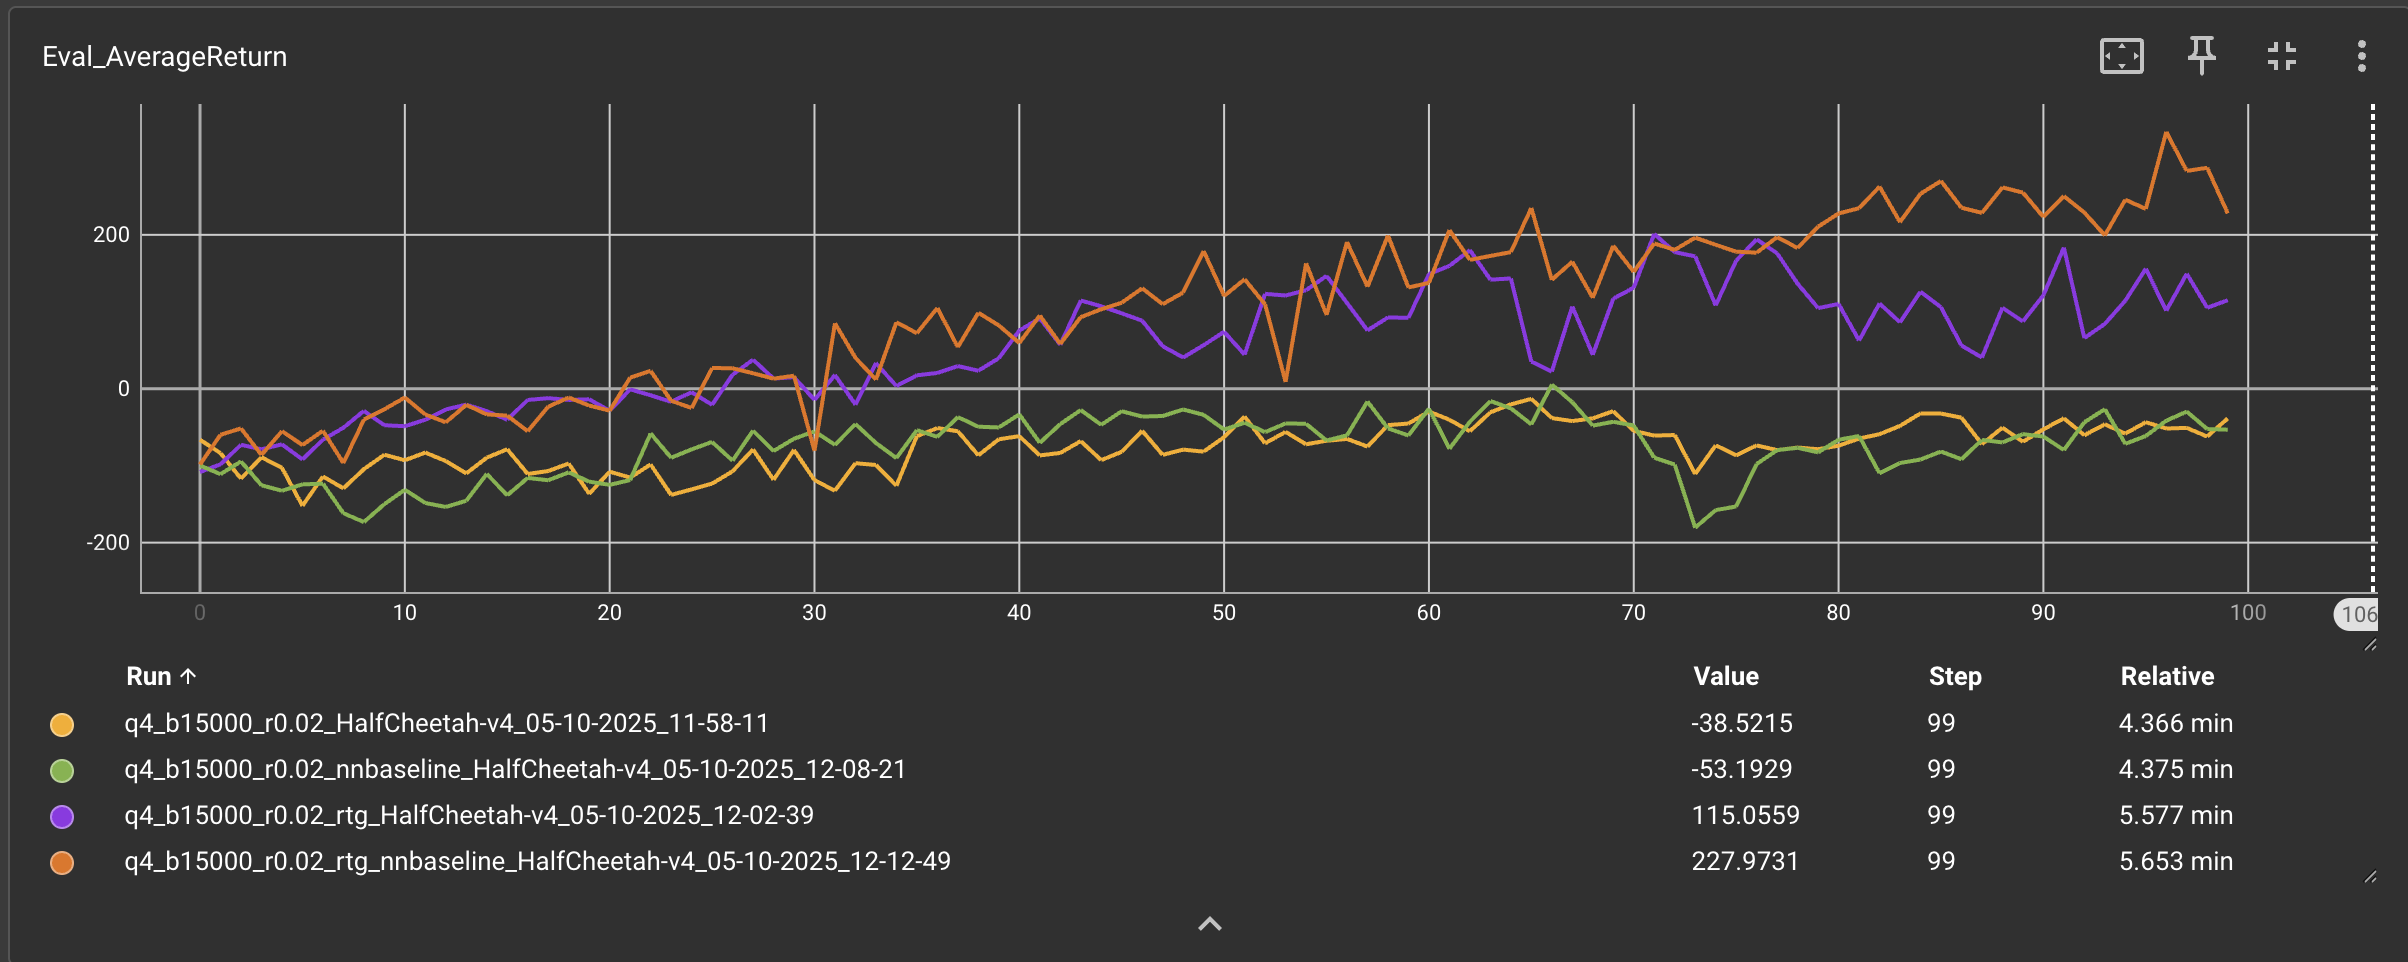
\includegraphics[height=8cm,width=\linewidth]{plots_submission/7_2_7_plot.png}
\end{answer}

\section{Implementing Generalized Advantage Estimation}

\subsection{Experiment 5 (Hopper) -- \lbrack4 points\rbrack}

\subsubsection{Configurations}
\begin{answer}[title=Q8.1.1,height=4cm,width=\linewidth]
\begin{minted}
[framesep=2mm, fontsize=\scriptsize, breaklines, escapeinside=||, mathescape=true]
{python}
# $\lambda \in [0,0.95,0.99,1]$
python rob831/scripts/run_hw2.py \
    --env_name Hopper-v4 --ep_len 1000
    --discount 0.99 -n 300 -l 2 -s 32 -b 2000 -lr 0.001 \
    --reward_to_go --nn_baseline --action_noise_std 0.5 --gae_lambda <|$\lambda$|> \
    --exp_name q5_b2000_r0.001_lambda<|$\lambda$|>
\end{minted}
\end{answer}

\subsubsection{Plot -- \lbrack2 points\rbrack}
\begin{answer}[title=Q8.1.2,height=10cm,width=\linewidth]
% TODO
\centering
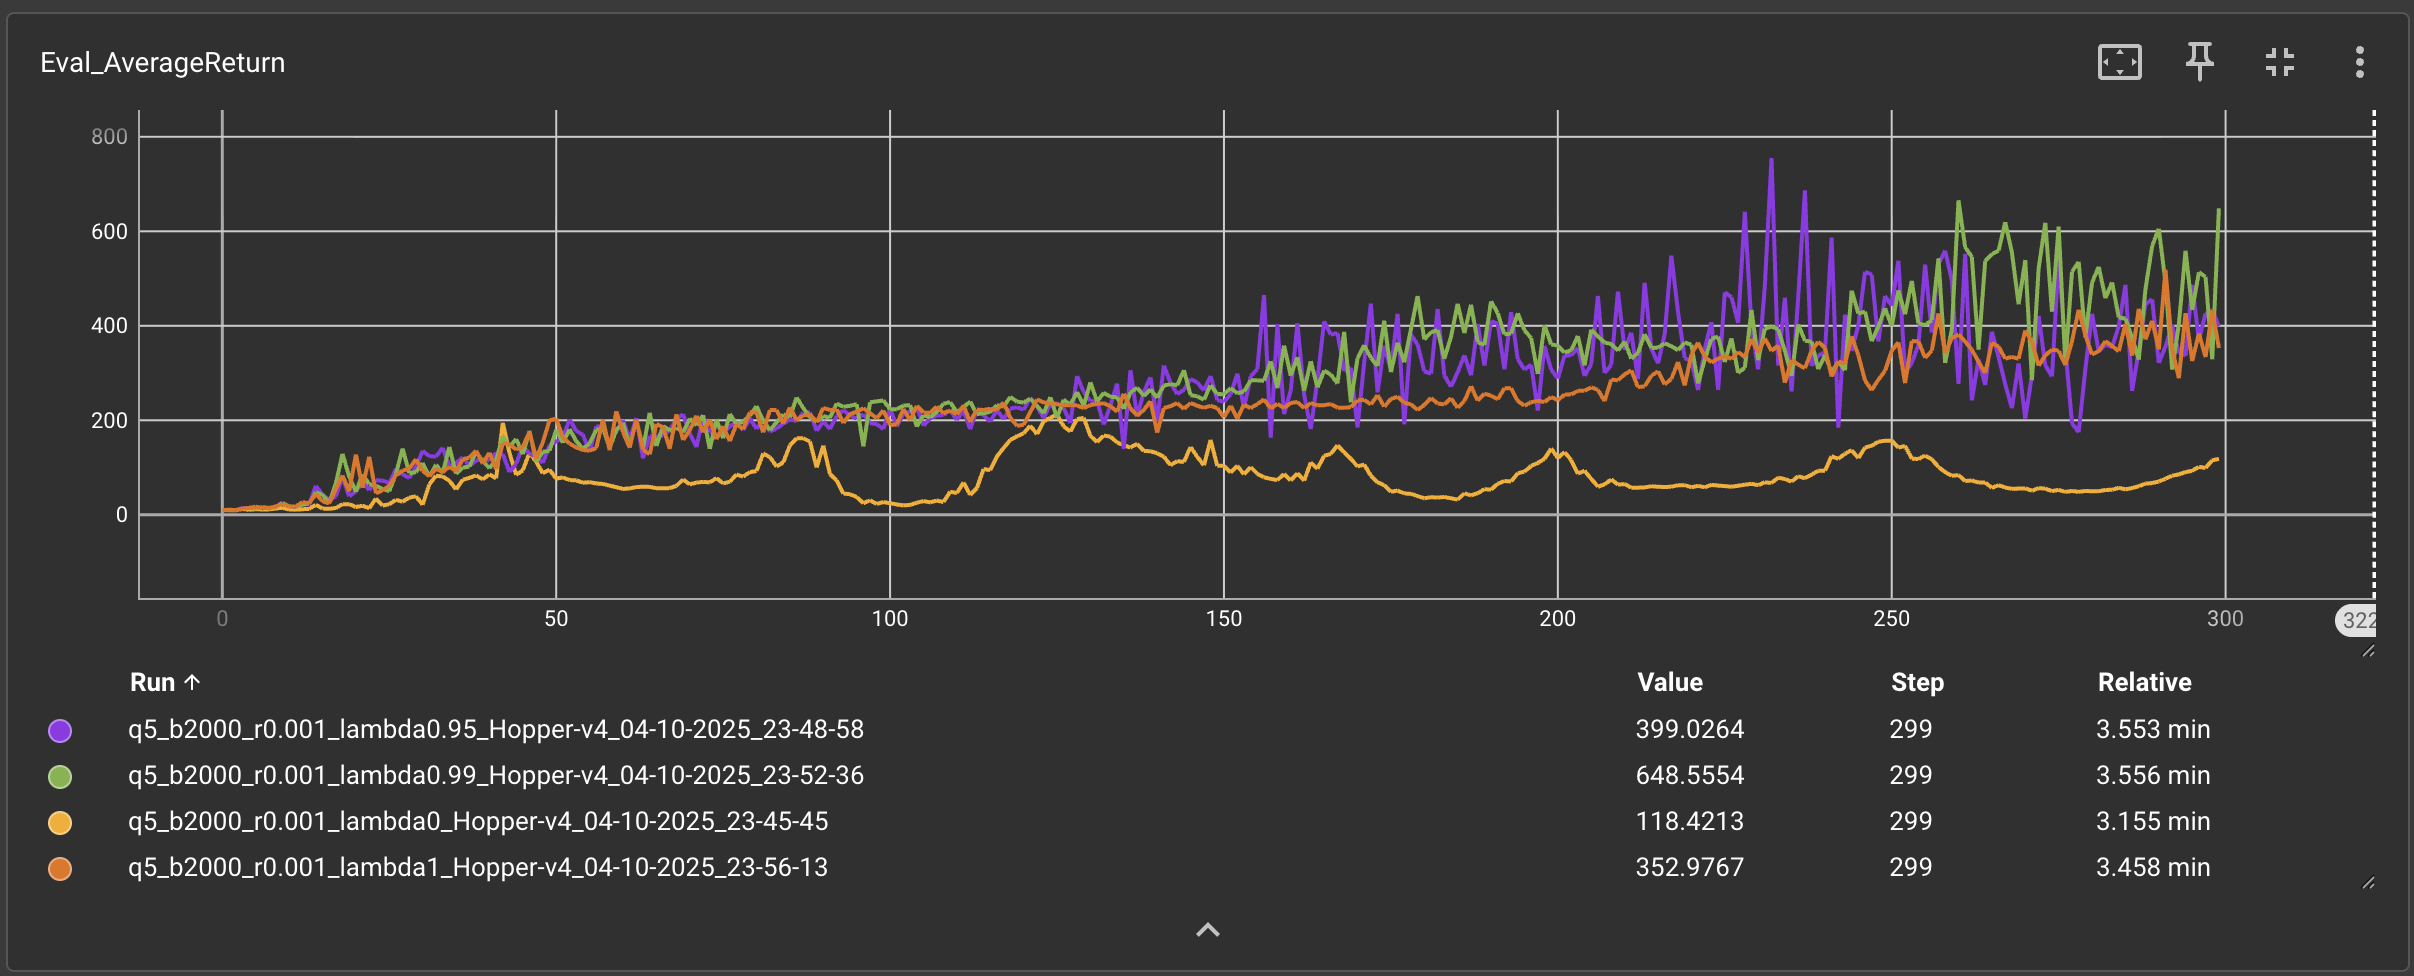
\includegraphics[height=8cm,width=\linewidth]{plots_submission/8_1_2_plot.png}
\end{answer}

\subsubsection{Describe how $\lambda$ affects task performance -- \lbrack2 points\rbrack}
\begin{answer}[title=Q8.1.3,height=4cm,width=\linewidth]
Generally, a higher $\lambda$ leads to a higher return and better performance.
\end{answer}

\clearpage

\section{More Bonus!}

\subsection{Parallelization -- \lbrack1.5 points\rbrack}
\begin{answer}[title=Q9.1,height=4cm,width=\linewidth]
% TODO (optional)
Difference in training time: 7.3 seconds
\vspace{1.0cm}
\begin{minted}
[framesep=2mm, fontsize=\scriptsize, breaklines]
{bash}
python rob831/scripts/run_hw2.py --env_name HalfCheetah-v4 \
-n 10 -b 10000 -lr 0.02 --exp_name test_cheetah_no_parallel

python rob831/scripts/run_hw2.py --env_name HalfCheetah-v4 \
--num_workers 4 -n 10 -b 10000 -lr 0.02 --exp_name test_cheetah_parallel
\end{minted}
\end{answer}

\subsection{Multiple gradient steps -- \lbrack1 points\rbrack}
\begin{answer}[title=Q9.1,height=14cm,width=\linewidth]
% TODO (optional)
\centering
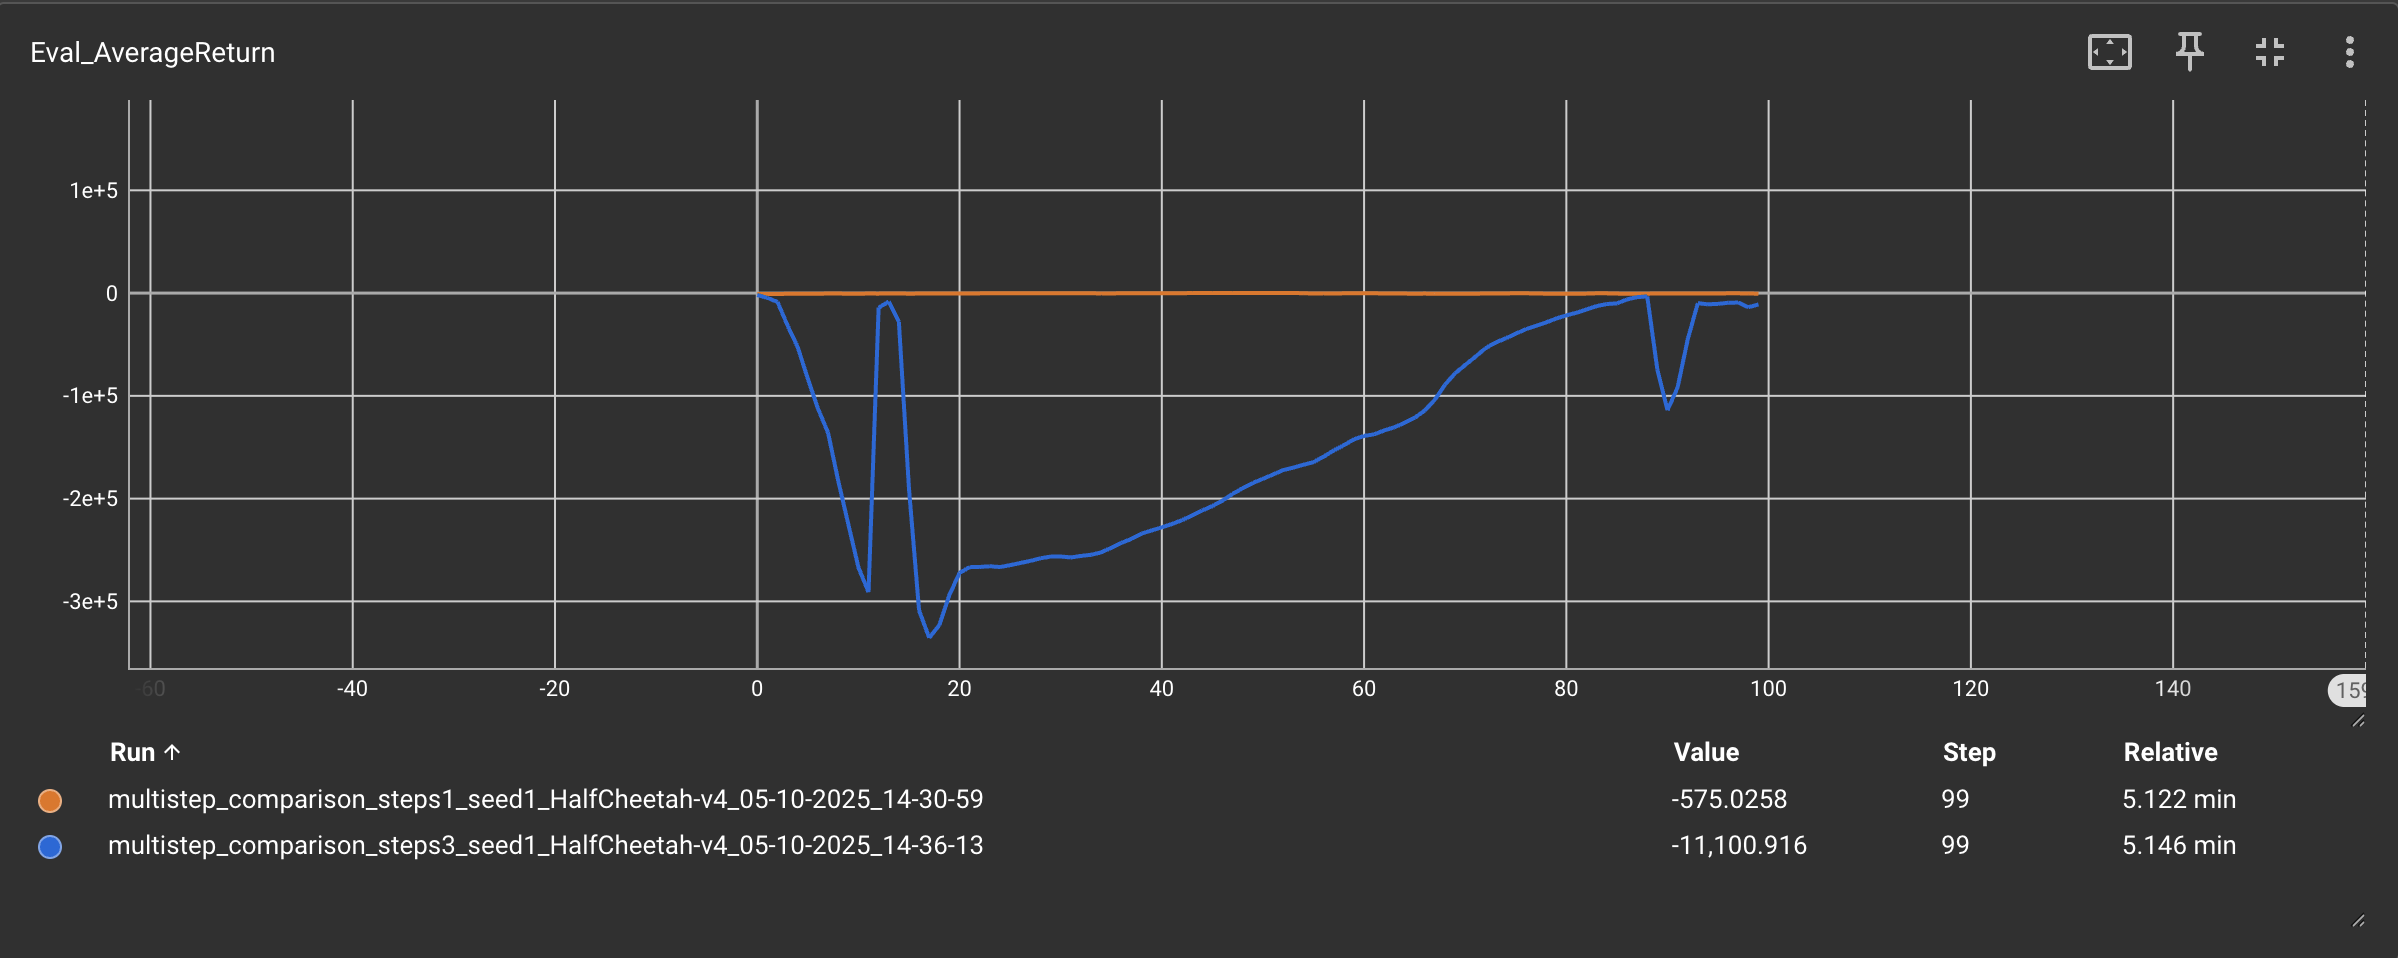
\includegraphics[height=8cm,width=\linewidth]{plots_submission/9_2_plot.png}

\vspace{1.0cm}
\begin{minted}
[framesep=2mm, fontsize=\scriptsize, breaklines]
{bash}
# Steps=1
python rob831/scripts/run_hw2.py --env_name "HalfCheetah-v4" --exp_name "multistep_comparison_steps1_seed1"
--n_iter 100 --batch_size 5000 --eval_batch_size 5000 --learning_rate 0.02 --discount 0.95 --n_layers 2 --size 64 --seed 1
--num_policy_gradient_steps_per_batch 1 --reward_to_go --nn_baseline --scalar_log_freq 1

# Steps=3
python rob831/scripts/run_hw2.py --env_name "HalfCheetah-v4" --exp_name "multistep_comparison_steps3_seed1"
--n_iter 100 --batch_size 5000 --eval_batch_size 5000 --learning_rate 0.02 --discount 0.95 --n_layers 2 --size 64 --seed 1
--num_policy_gradient_steps_per_batch 3 --reward_to_go --nn_baseline --scalar_log_freq 1
\end{minted}

\end{answer}

\end{document}
